% 买房还是租房 —— XeLaTeX 编译: cd paper && xelatex paper.tex && xelatex paper.tex
\documentclass[11pt,a4paper]{ctexart}
\usepackage[margin=2.6cm]{geometry}
\usepackage{graphicx}
\usepackage{booktabs}
\usepackage{amsmath}
\usepackage{float}
\usepackage{tabularx}
\usepackage{caption}
\PassOptionsToPackage{hyphens}{url}
\usepackage[colorlinks=true,linkcolor=black,urlcolor=blue,citecolor=black]{hyperref}
\expandafter\def\expandafter\UrlBreaks\expandafter{\UrlBreaks%
  \do\a\do\b\do\c\do\d\do\e\do\f\do\g\do\h\do\i\do\j\do\k\do\l\do\m%
  \do\n\do\o\do\p\do\q\do\r\do\s\do\t\do\u\do\v\do\w\do\x\do\y\do\z%
  \do\0\do\1\do\2\do\3\do\4\do\5\do\6\do\7\do\8\do\9\do\_\do\-}
\graphicspath{{../figures/}}
\captionsetup{font=small,labelfont=bf}
\setlength{\parskip}{0.35em}

\title{\bfseries 买房还是租房？\\ \Large ——用150年跨国历史把预测题变成概率题}
\author{}
\date{初稿 · 2026年8月}

\begin{document}
\maketitle

\begin{abstract}

\noindent ``买房还是租房''争论不休，是因为账里有三个未来量——房价涨速、租金涨速、替代投资收益率——没人能预测。本文把决策变量分成三层（可直接观察的、半可预测的、不可约不确定的），用 Jordà-Schularick-Taylor 宏观历史数据库（18 国、1870--2020）为不可观察的量建立经验分布，把``买房是否划算''重述为两个可查证的问题：\textbf{(i) 给定可观察的租售比、利率与成本，买房打平需要多高的真实房价年涨幅 $g^*$；(ii) 这个涨幅在 150 年 $\times$ 16 国的历史中出现过多大比例。}实证部分确认：真实房价长期涨幅很低（1870--1950 年中位数 +0.3\%/年，1950 年后 +2.3\%/年）；住房总回报约 7\%/年中约五个百分点来自租金；期初租售比偏离负向预测未来十年房价，但按重叠窗口修正后仅勉强显著（双向聚类 t=$-$2.08，p$\approx$0.055；五年期 t=$-$1.71，不显著），R²$\approx$2\%——弱预测力本身即是``输出概率而非点估计''的理由。算法遍历全部历史窗口生成买房胜率，并以国家为整群的自助法配 95\% 区间。租金收益率 1.8\%、按揭 4\% 的市场，持有十年买房胜率约 20\%（区间 [14, 26]）；租金收益率 5.5\%、按揭 6.5\% 的市场约 60\%（[51, 68]）；持有期短于 5 年时租房几乎总是胜出。2026 年中国的案例研究（第 8 节）显示，买租天平较 2021 年大幅回摆：二线省会成为唯一金融账基本打平的画像，一线仍偏租但期望代价从 30\%+ 房价缩小到约一成。

\end{abstract}

\section{引言}

如果有人能准确告诉你未来十年的房价涨幅、租金涨幅和替代投资收益率，``买房还是租房''就只是一道初中算术题。争论的全部来源，是这三个数没人知道。对此常见的两种反应都不能令人满意：假装知道——挑一个``合理假设''代入，得到看似精确、实则由假设驱动的结论；或放弃计算——``看个人情况''，把一个大部分可以量化的问题交给情绪。

本文走第三条路：\textbf{承认这三个量不可精确预测，但拒绝承认它们完全不可知。} 150 年、18 个发达经济体的完整记录告诉我们这些量的经验分布长什么样、被什么可观察变量所条件化。问题于是从``预测未来''降格为``查历史频率''：买房打平所需的涨幅，在历史上、在当前这样的估值水平之后，出现过多少次？代价是答案从``该买/该租''变成``买房胜率 62\%''——但这正是这个问题诚实答案的形态，而且城市之间的差别大到足以指导行动（第 7、8 节）。

\section{模型：这道算术题的精确形式}

比较两条路径在持有期 $T$ 年末的净财富。两条路径每年花同样多的钱（取两者现金流出的较大值），少花的一方把差额投入替代资产——比较的是``同一笔钱走两条路''。

\textbf{买}：首付 $d \cdot P_0$，贷款 $(1-d)P_0$ 以利率 $i$ 等额本息 $n$ 年；每年付月供与持有成本 $c \cdot P_t$；期初付交易成本 $\kappa_b P_0$；期末以 $P_T$ 卖出，付 $\kappa_s P_T$，清偿贷款余额。

\textbf{租}：租住同等房屋，年租金 $R_t = ry \cdot P_0 (1+g_R)^{t-1}$（$ry$ 为当前租金收益率，即租售比的倒数）；把首付、交易成本与每年买租现金流差额投入替代资产，税后年化收益 $r$。

期末财富差 $\Delta(T) = W_{\text{买}} - W_{\text{租}}$ 是房价涨幅 $g_P$ 的单调增函数；\textbf{盈亏平衡涨幅} $g^*$ 是使 $\Delta(T)=0$ 的 $g_P$。现金流按年频、年初发生，期末结算。这个终值比较与使用者成本框架（Poterba 1984; Himmelberg, Mayer \& Sinai 2005）在一期近似下等价：买入划算当且仅当

\begin{equation*}
ry > u \equiv i + c + \kappa/T - g_P.
\end{equation*}

终值形式的好处是精确处理杠杆、摊销、租金增长与交易成本的时间结构，并让``锁定名义月供''显式出现——通胀上行时租金与房价上移而月供不变，业主天然持有一份通胀对冲（Sinai \& Souleles 2005）。

\section{变量三分法}

模型输入按认识论地位分三层，这是全文的方法论骨架：

\begin{itemize}\itemsep0.2em
\item \textbf{A 层——决策时刻直接可观察}：当前租金收益率 $ry$、按揭利率 $i$、首付比例 $d$、交易成本 $\kappa_b, \kappa_s$、持有成本 $c$、持有期 $T$。精确代入。
\item \textbf{B 层——半可预测}：未来房价涨幅部分地被期初估值条件化（4.3 节）；租金涨速长期贴着当地收入（4.5 节）。
\item \textbf{C 层——不可约的不确定}：替代投资收益率、通胀体制、政策冲击。只能以历史分布处理。
\end{itemize}

关键观察：\textbf{争议最大的量（房价涨幅）恰好拥有最好的可观察代理（租售比）}。

\section{历史证据：六个典型事实}

数据为 JST Macrohistory Database R6（18 国 1870--2020 年，含 Knoll, Schularick \& Steger 2017 的房价序列与 Jordà 等 2019 的回报序列）。恶性通胀年份（|通胀|>50\%）剔出回报统计。全部数字由 \texttt{analysis/stylized\_facts.py} 生成。

\textbf{关于样本量。}数据库有 18 国，但各事实建立在不同子样本上：事实一的真实房价面板为 \textbf{13 国}（1870--1950 年的中位数只有 \textbf{12 国}）；事实三、四、六与\textbf{全部算法输出}依赖租金收益率序列，为 \textbf{16 国}（缺加拿大、爱尔兰）。凡称``历史频率''``胜率''处，经验基础都是这 16 国。

\subsection{事实一：真实房价的长期涨幅很低，且集中在 1950 年之后}

\begin{figure}[H]\centering
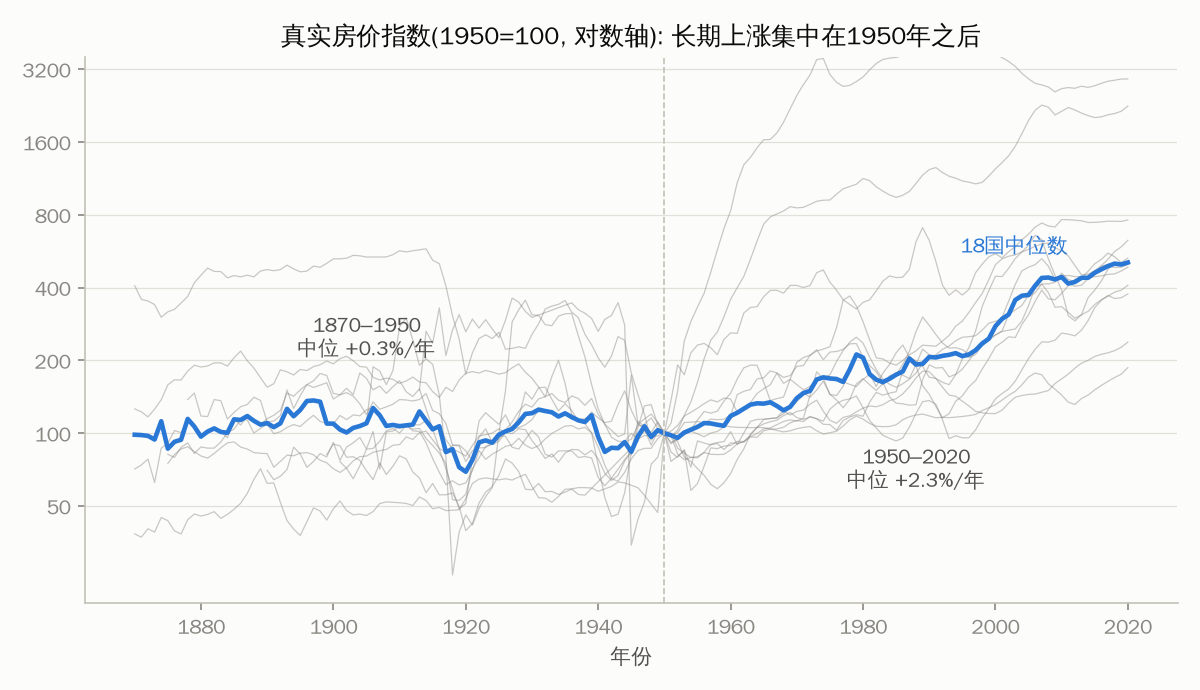
\includegraphics[width=0.92\linewidth]{fig1_real_house_prices.png}
\caption{真实房价指数（1950=100，对数轴，13 国面板）。}
\end{figure}

真实房价指数（1950=100，13 国面板）的跨国中位数，1870--1950 年的年化涨幅只有 \textbf{+0.3\%}（该时段可得 12 国）——三代人的时间里房价基本只跟着通胀走。1950--2020 年升至 \textbf{+2.3\%/年}，全样本 1870--2020 为 \textbf{+1.2\%/年}，战后上涨的约八成来自地价（Knoll 等 2017）。``房价长期必然大幅跑赢通胀''的先验与 1950 年前的八十年不符；战后体制是否延续是不可知的 C 层问题，而且即便延续，+2.3\% 也远低于多数购房者的心理预期。

\subsection{事实二：住房回报的大头是租金，不是涨价}

\begin{figure}[H]\centering
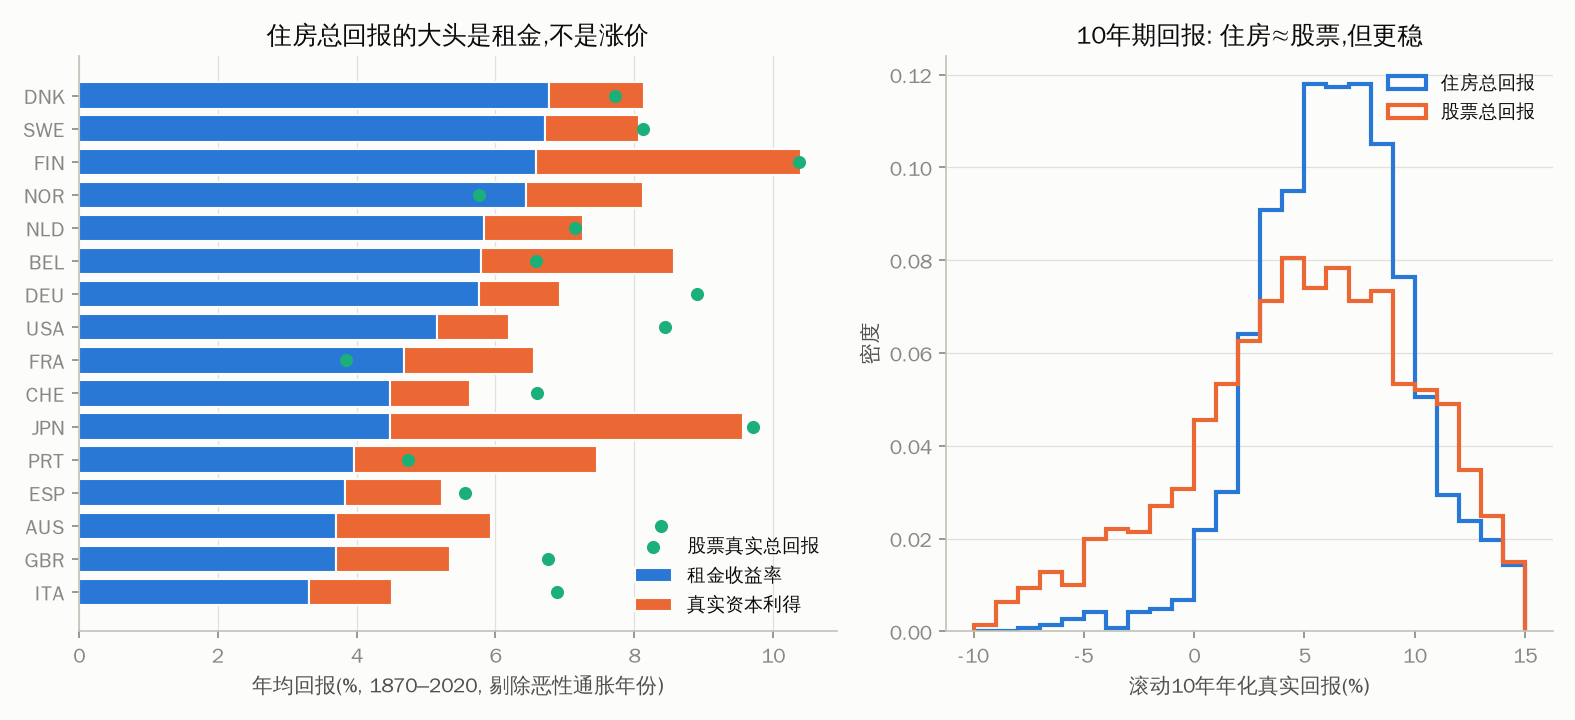
\includegraphics[width=\linewidth]{fig2_return_decomposition.png}
\caption{左：各国住房年均回报的分解（1870--2020）；右：滚动 10 年年化真实回报分布。}
\end{figure}

各国 1870--2020 年均：租金收益率 \textbf{5.1\%}，真实资本利得 \textbf{2.0\%}，住房真实总回报 \textbf{7.0\%}——与股票的 \textbf{7.2\%}几乎相同（Jordà 等 2019），而离散度更低（滚动十年标准差 3.8\% 对 5.8\%）。\textbf{自住买房``赚''的可靠部分是省下的租金，投机部分才是涨价}：租金收益率 5\% 的市场，买房不需要房价涨也划算；租金收益率 1.5\% 的市场，买房的全部逻辑都押在涨价上。

\subsection{事实三：租售比偏离负向预测未来房价——方向可靠，力度温和}

\begin{figure}[H]\centering
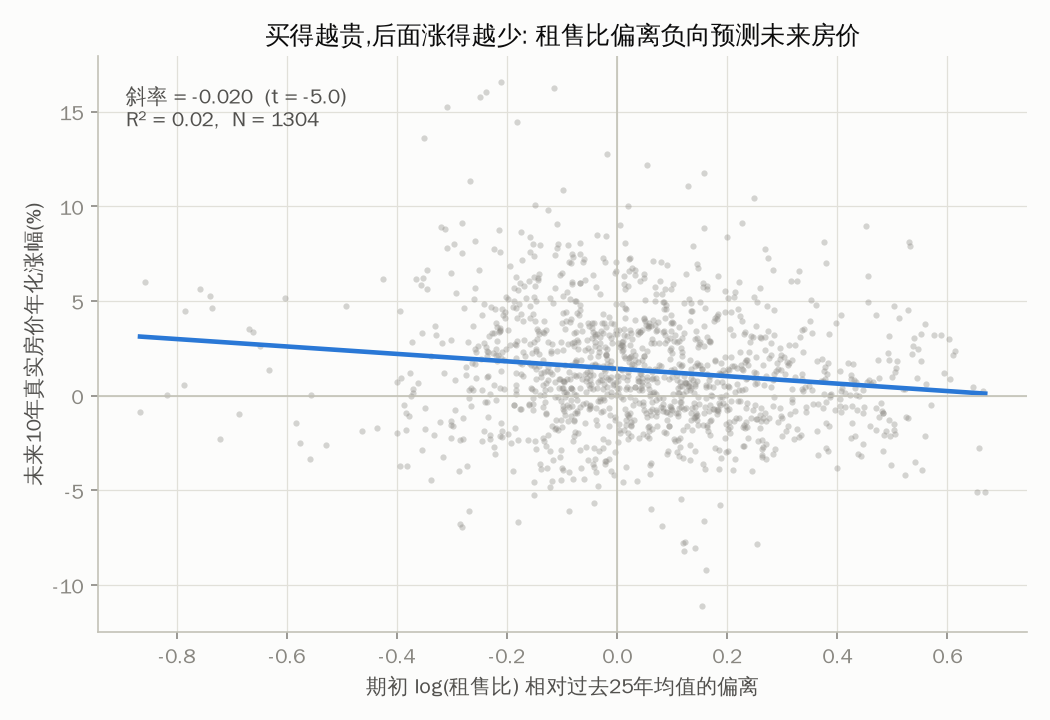
\includegraphics[width=0.8\linewidth]{fig3_mean_reversion.png}
\caption{期初 $\log$(租售比) 相对过去 25 年均值的偏离 vs 未来 10 年真实房价年化涨幅。}
\end{figure}

以``log 租售比相对本国过去 25 年均值的偏离''为期初估值代理（决策时刻实时可算），对未来 10 年真实房价年化涨幅做池化回归：斜率 \textbf{$-$0.020}（N=1304，16 国）；5 年期 $-$0.023（N=1421）。方向与 Gallin（2008）一致：买得越贵，后面涨得越少。

\textbf{但显著性必须按重叠窗口修正后报告。}相邻十年窗口共享九年数据，各国又受同一轮全球周期驱动，朴素 OLS 的标准误被系统性低估。以聚类稳健标准误重算（\texttt{analysis/uncertainty.py}）：

\begin{table}[H]\centering\small
\begin{tabular}{lcc}
\toprule
标准误口径 & 10 年期 t & 5 年期 t \\
\midrule
朴素 OLS & $-$5.05 & $-$4.22 \\
按国家聚类 & $-$2.15 & $-$1.79 \\
按起始年聚类 & $-$3.77 & $-$2.97 \\
双向聚类（国家 $\times$ 起始年） & \textbf{$-$2.08} & \textbf{$-$1.71} \\
\bottomrule
\end{tabular}
\end{table}

以双向聚类为准（t(G$-$1)、G=16）：\textbf{十年期 p$\approx$0.055，五年期 p$\approx$0.11}——十年尺度勉强够到显著性门槛，五年尺度与零无法区分；朴素 OLS 的 t$\approx$$-$5 是窗口重叠制造的假象。而且 \textbf{R² 只有约 2\%}：期初估值移动未来涨幅的均值，却远不能锁定它。这是本文的核心方法论证据——最好的可观察代理也只有温和的预测力，任何输出点估计的买租计算器都在假装拥有不存在的信息。

\subsection{事实四：未来涨幅的历史分布——算法的查询表}

\begin{figure}[H]\centering
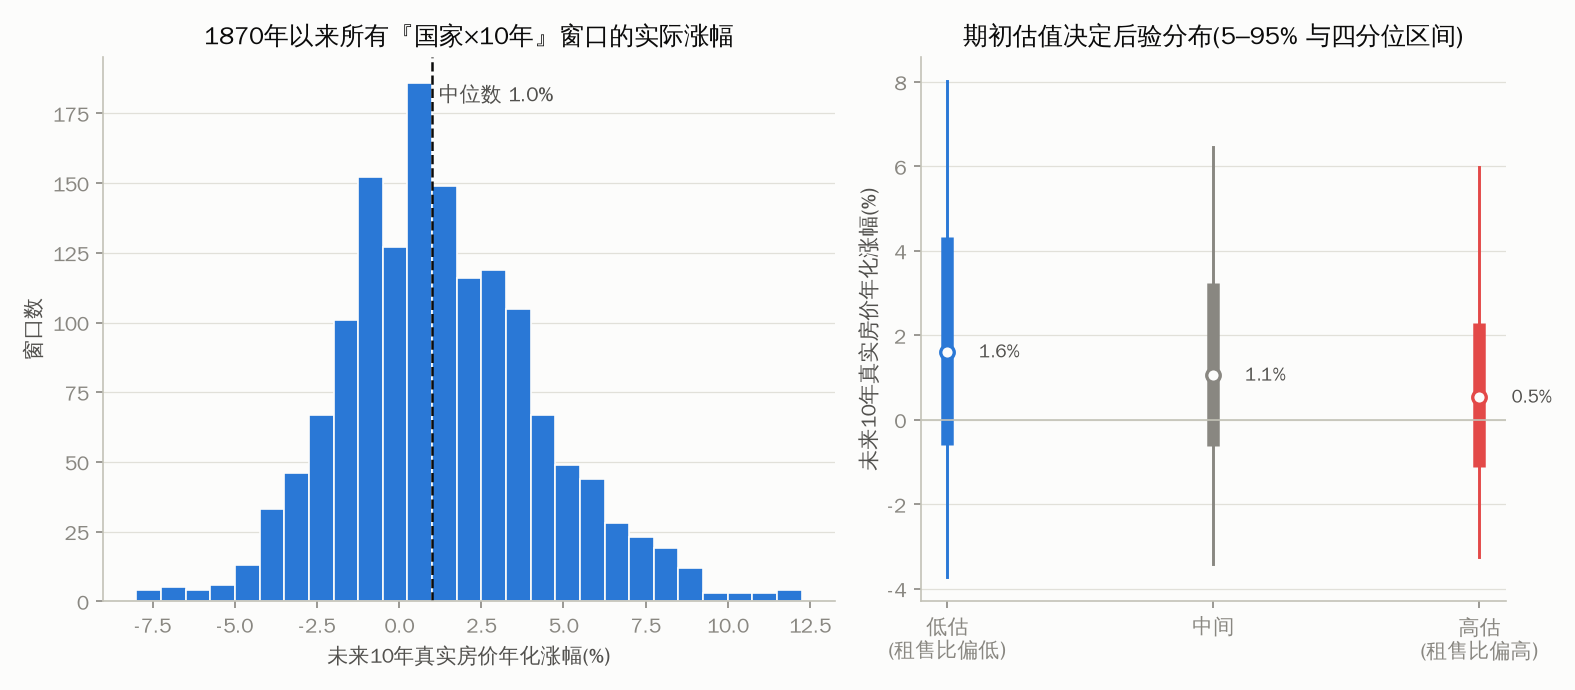
\includegraphics[width=\linewidth]{fig4_growth_distribution.png}
\caption{左：全部``国家$\times$10 年''窗口的真实房价年化涨幅；右：按期初估值三分位的条件分布。}
\end{figure}

全部 1510 个``国家 $\times$ 10 年''窗口（16 国）中，真实房价年化涨幅的分布：

\begin{table}[H]\centering\small
\begin{tabular}{lccccc}
\toprule
分位 & 5\% & 25\% & 50\% & 75\% & 95\% \\
\midrule
年化真实涨幅 & $-$3.4\% & $-$0.7\% & \textbf{+1.0\%} & +3.2\% & +7.1\% \\
\bottomrule
\end{tabular}
\end{table}

\begin{table}[H]\centering\small
\begin{tabular}{lcccccc}
\toprule
门槛(年化真实) & $\geq$0\% & $\geq$1\% & $\geq$2\% & $\geq$3\% & $\geq$4\% & $\geq$5\% \\
\midrule
历史频率 & 66\% & 50\% & 38\% & 27\% & 18\% & 12\% \\
95\% 区间 & [61, 70] & [46, 55] & [32, 43] & [22, 32] & [14, 22] & [8, 16] \\
\bottomrule
\end{tabular}
\end{table}

\textbf{频率本身也是估计量。}背后只有 16 个国家且窗口高度重叠，因此以国家为整群（block）有放回抽样得到 95\% 区间，宽度约 $\pm$4--5 个百分点——此后引用这些频率，都按``十位数可读、个位数不可读''使用。

按期初估值三分位条件化后分布整体平移：低估组中位 \textbf{+1.6\%}、十年下跌概率 31\%（[23, 39]）；高估组中位 \textbf{+0.5\%}、下跌概率 \textbf{42\%}（[35, 48]）。但两组下跌概率之差 \textbf{10.6 个百分点的 95\% 区间为 [$-$0.8, +21.3]}（单边 p$\approx$0.03）：估值条件化的\textbf{方向}站得住，\textbf{强度}只够支撑一次温和的先验移动，不足以支撑``高估的市场必然下跌''。

这张表就是算法的核心：把``你认为房价会涨多少''这个无法验证的信念，换成``你需要的涨幅在历史上出现过多少次''这个可以验证的事实。

\subsection{事实五：真实租金增速低于且贴着收入增速}

\begin{figure}[H]\centering
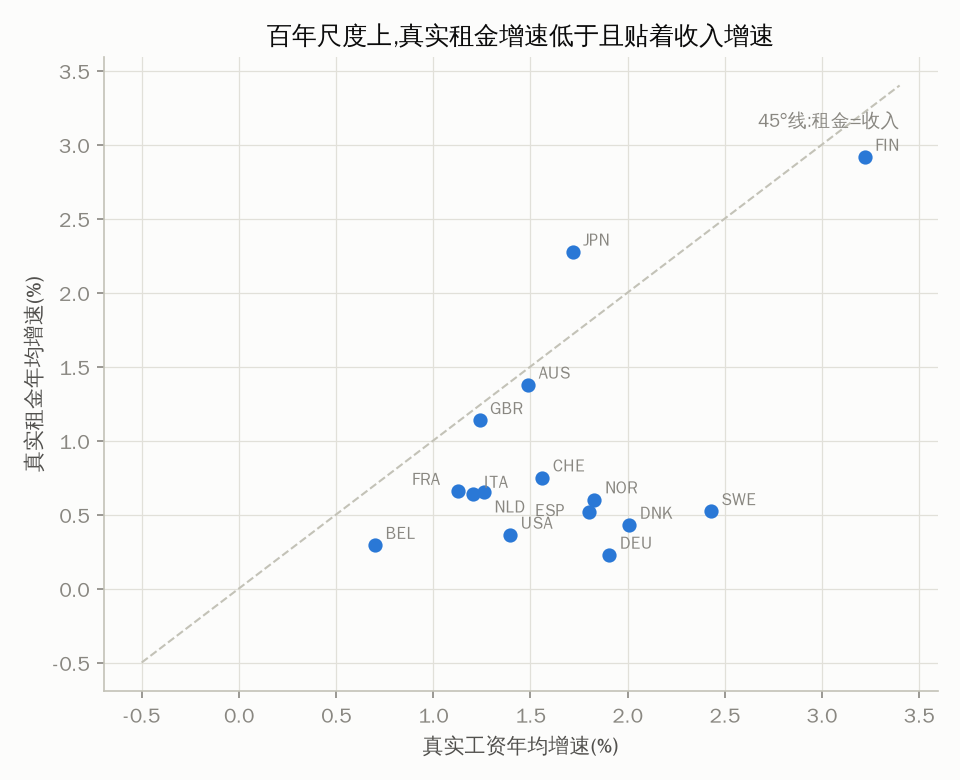
\includegraphics[width=0.62\linewidth]{fig5_rent_vs_income.png}
\caption{各国百年尺度真实租金增速 vs 真实工资增速。}
\end{figure}

各国百年尺度的真实租金年均增速平均 \textbf{+0.9\%}，系统性低于真实工资增速（\textbf{+1.7\%}），所有国家都落在 45$^\circ$ 线下方。``当地名义收入增速''是租金涨速一个略偏保守的上界锚。

\subsection{事实六：持有期短是买方无法克服的劣势}

买卖交易成本各国合计约 5--10\%。持有 3 年时即便房价与投资同速增长，租房仍稳定胜出（第 7 节画像 C）。这是全文最不依赖预测的结论：\textbf{预期五年内可能搬家的人，租。}

\section{代理变量：问题的答案}

回到出发点——``能否找到相对准确的代理变量？''。按（可观察性 $\times$ 预测力）排序：

\begin{enumerate}\itemsep0.2em
\item \textbf{当前租金收益率}——决定买方现金流账的底色（事实二），单个最重要且完全可观察；
\item \textbf{租售比相对本地历史常态的偏离}——温和地条件化未来涨幅分布（事实三、四），只应当作先验的小幅移动而非判据；
\item \textbf{真实按揭利率}——使用者成本的最大项，合同可锁定；
\item \textbf{本地收入增速}——租金涨速的锚（事实五）；
\item \textbf{持有期}——个人变量，但作用完全确定（事实六）。
\end{enumerate}

代理集内部再分层：\textbf{第 (1)、(3)、(5) 项可观察且作用确定，构成结论的骨架；第 (2)、(4) 项只是对分布的温和修正}——它们把十年下跌概率在 31\% 与 42\% 之间移动，却不能把分布收窄成一个数。一个只用前三项的粗糙判断，比一个把第 (2) 项当作强信号的精致判断更可靠。

\section{算法}

\begin{center}\small
\begin{tabular}{ll}
\toprule
输入 & A 层观察值: $ry, i, d, n, \kappa_b, \kappa_s, c, T$；可选: 本市历史常态租金收益率 \\
\midrule
第 1 层 确定性核心 & 终值财富比较（第 2 节模型），A 层精确代入 \\
第 2 层 盈亏平衡 & 解 $g^*$：使买 = 租的房价涨幅（brentq） \\
第 3 层 历史频率 & $P(\text{实际涨幅} \geq g^* \mid \text{持有期})$——查事实四的窗口表；\\
 & 若给出本市历史常态租售比 $\rightarrow$ 按估值三分位条件化 \\
第 4 层 历史全量求值 & 遍历同持有期（可选同估值组）的每一个历史窗口，取 \\
 & （$g_{\text{房}}, g_{\text{租}}, r_{\text{股}}, r_{\text{债}}$, 通胀）的联合实现值代入模型 \\
 & $\rightarrow$ P(买优于租)，财富差分布 \\
第 5 层 不确定性 & 以国家为整群（block）有放回抽样，给第 3、4 层的 \\
 & 每个概率配 95\% 区间 \\
\midrule
输出 & $g^*$、历史频率（含区间）、买房胜率（含区间）、期末财富差的 90\% 区间 \\
\bottomrule
\end{tabular}
\end{center}

设计要点有三。\textbf{不假设参数分布}：直接取真实历史窗口的联合实现值，变量间的相关结构（通胀推高名义租金与房价而月供锁定；股房共动）原样保留。\textbf{全量而非抽样}：同持有期的窗口池只有数百到一千余个，逐个求值即得精确胜率。\textbf{不确定性以国家为整群}：把整个国家作为不可分的 block 重抽，同时吸收窗口重叠与国别内相关；block 只有 16 个，区间偏保守。第 3 层只动房价一个变量，直观可核；第 4 层让所有 B/C 层变量同时动——高租金收益率市场中后者的胜率（60\%）高于前者（51\%），正是租金增长与通胀对冲两条买方优势，但两者区间大幅重叠，只宜定性解读。

\begin{figure}[H]\centering
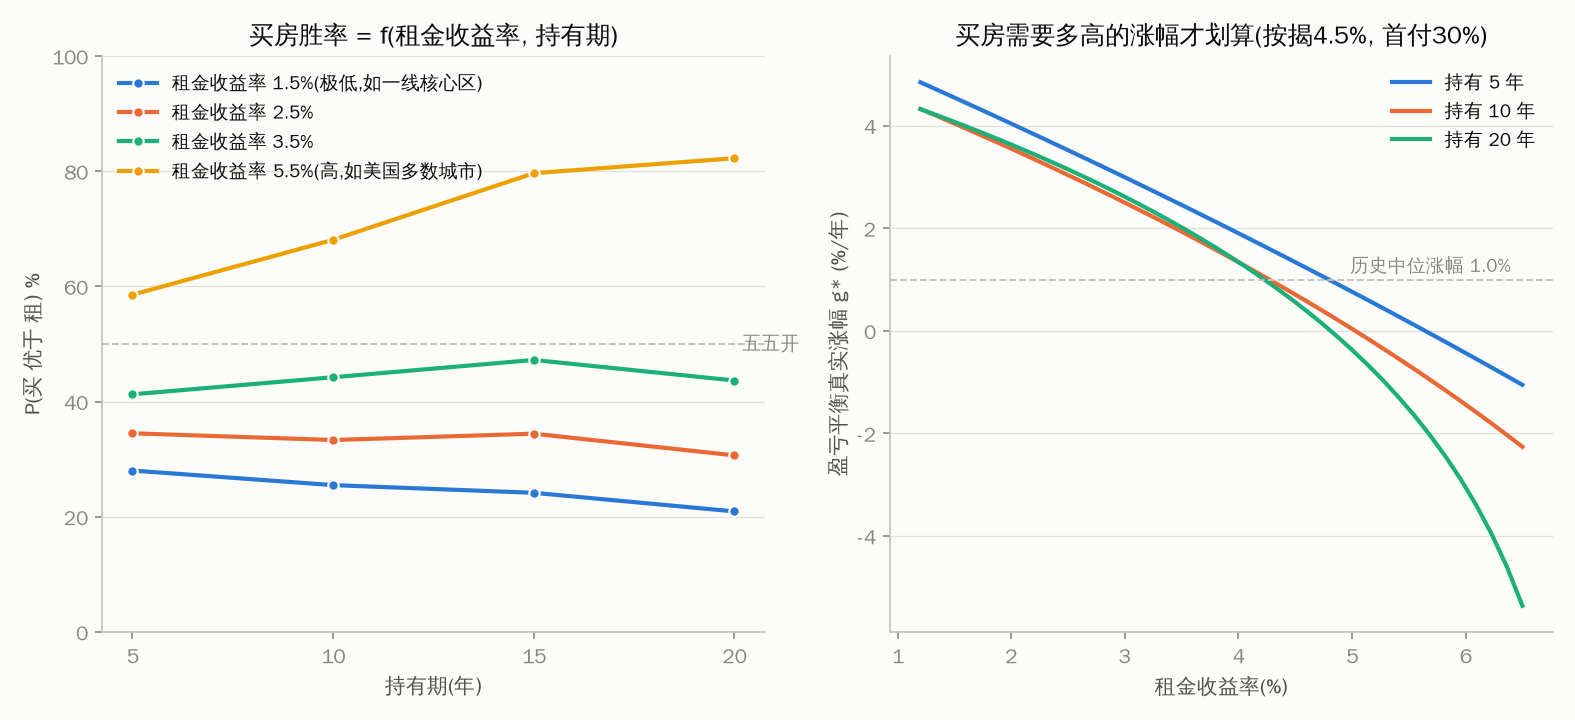
\includegraphics[width=\linewidth]{fig6_algorithm.png}
\caption{左：买房胜率随租金收益率与持有期变化；右：盈亏平衡真实涨幅 $g^*$（按揭 4.5\%、首付三成）。}
\end{figure}

上图右格给出一个可携带的经验法则：\textbf{按揭 4.5\%、首付三成时，租金收益率约 4.5\% 是``买房不靠涨价也划算''的分水岭}（$g^*$ 降到历史中位涨幅 1.0\% 以下）；左格显示租金收益率 5.5\% 的市场持有二十年买房胜率约 82\%，租金收益率 1.5\% 的市场持有再久也不超过 30\%。

\section{案例应用}

三个风格化画像（由 \texttt{python3 analysis/cases.py} 生成并写入 \texttt{data/derived/cases.json}，测试锁定其与本表一致；方括号为 95\% 区间）：

\begin{table}[H]\centering\small
\begin{tabularx}{\textwidth}{lXXX}
\toprule
 & A: 低租售比大城市 & B: 高租售比市场 & C: 短持有期 \\
\midrule
参数 & ry 1.8\%（历史常态 2.2\%）, 按揭 4.0\%, 持有 10 年 & ry 5.5\%（处于自身常态）, 按揭 6.5\%, 持有 10 年 & ry 3.0\%, 按揭 3.5\%, 持有 3 年 \\
盈亏平衡真实涨幅 g* & \textbf{+3.5\%/年 $\times$10年} & \textbf{+0.9\%/年} & +3.2\%/年 $\times$3年 \\
历史频率(无条件) & 22\% [19, 26] & 51\% [46, 56] & 32\% [29, 35] \\
历史频率(按估值条件化) & \textbf{15\%} [9, 23]（高估组） & 52\% [44, 61]（中间组） & — \\
P(买优于租) & \textbf{20\%} [14, 26] & \textbf{60\%} [51, 68] & 38\% [34, 42] \\
财富差中位(占房价,真实) & $-$32\% & +9\% & $-$5\% \\
90\% 区间 & [$-$113\%, +39\%] & [$-$61\%, +88\%] & [$-$30\%, +28\%] \\
\bottomrule
\end{tabularx}
\end{table}

画像 A 接近跌价前的中国一线城市：打平需要连续十年 3.5\% 的真实涨幅，全部历史中只有约两成窗口做到过，类似的高估值起点之后约一成半。画像 B 接近美国多数都会区：几乎不需要涨幅就划算。画像 C 展示事实六：即便利率低、估值中性，三年持有期就足以让买方在中位情形下亏掉 5\% 的房价。

A 与 B 的胜率区间（[14, 26] 与 [51, 68]）相隔很远，\textbf{这个差别是数据能支撑的}；A 的 20\% 与另一个 25\% 的画像之间，数据支撑不了任何区分。\textbf{这个问题没有普适答案，但有普适算法。}

\section{案例研究：2026 年的中国——分城市、分人群}

本节把算法应用于 2026 年年中的中国，参数取自公开数据（来源见文末），并做三处制度修正：\textbf{(i)}租房者的替代投资收益率固定为中国居民实际可得的水平；\textbf{(ii)}中国按揭是 LPR 浮动利率，因此把窗口通胀固定在现值 0.5\%——若照搬历史通胀（窗口平均约 3.5\%）并锁定名义月供，等于凭空授予买方一份美式固定利率按揭独有的通胀对冲，会把胜率系统性抬高约 15--20 个百分点；\textbf{(iii)}三四线城市叠加人口与流动性的场外修正。\textbf{本节是金融账的估算，不构成投资建议；所有参数都可在 \texttt{analysis/china\_2026.py}或网页计算器里改成你自己的数字。}

\subsection{2026 年的输入变量}

\begin{table}[H]\centering\small
\begin{tabularx}{\textwidth}{lXX}
\toprule
变量 & 2026 年取值 & 说明 \\
\midrule
按揭利率 & \textbf{3.1\%}（新发放加权平均，2026Q2） & 5 年期 LPR 3.5\%（2026-08 连续 15 个月未动）；公积金 5 年以上 2.6\% \\
租金收益率 & 北京 1.64 / 上海 1.95 / 广州 1.87 / 深圳 1.82（2025-11）；二线平均 \textbf{2.36}（2026-03，杭苏约 2.0，成都武汉 >2.3）；三四线约 2.2 & 较 2021 年顶部普遍修复 0.3--0.8 个百分点（房价下跌所致） \\
市场状态 & 2026 上半年百城二手房价累跌 2.9\%，跌幅收窄；沪深二手转涨 & 核心城市二手价较 2021 高点累计跌约 20--30\%，市场筑底 \\
物价与利率环境 & CPI $\approx$ 0；10 年期国债 \textbf{1.73\%} & 名义按揭 3.1\% $\approx$ \textbf{真实利率 3\%}，并不低；租房者可得收益率：存款 $\sim$1.3\%、理财 2--2.5\% \\
交易与持有 & 买入成本约 2.5\%（含中介）；满五唯一卖出约 1.5\%；无房产税，持有成本约 0.7\%/年 & 首付最低 15--20\%，本节按 30\% 计算 \\
\bottomrule
\end{tabularx}
\end{table}

与 2021 年相比，三个关键变量都朝有利于买方的方向移动：房价跌了两到三成、按揭利率从 5.3\% 降到 3.1\%、租房者的投资收益率从``理财 4--5\%''塌缩到``1 字头''。2021 年顶部的一线城市打平需要\textbf{连续十年 +2.8\% 的真实涨幅}，高估起点后的历史频率只有 \textbf{22\%}——此后房价的实际走势与之相符；同样的城市在 2026 年只需要 \textbf{+1.6\%}，条件频率升到 34\%。

\subsection{分城市结果}

四类城市画像、两类租房投资者（保守型：存款/国债/理财，真实收益 1.5\%；均衡型：含权益或全球配置，真实 3\%），持有 10 年，估值按各城相对自身 25 年常态的偏离条件化（所有画像都落在``高估组''；各城``常态''是假设，敏感性见本节末）：

\begin{figure}[H]\centering
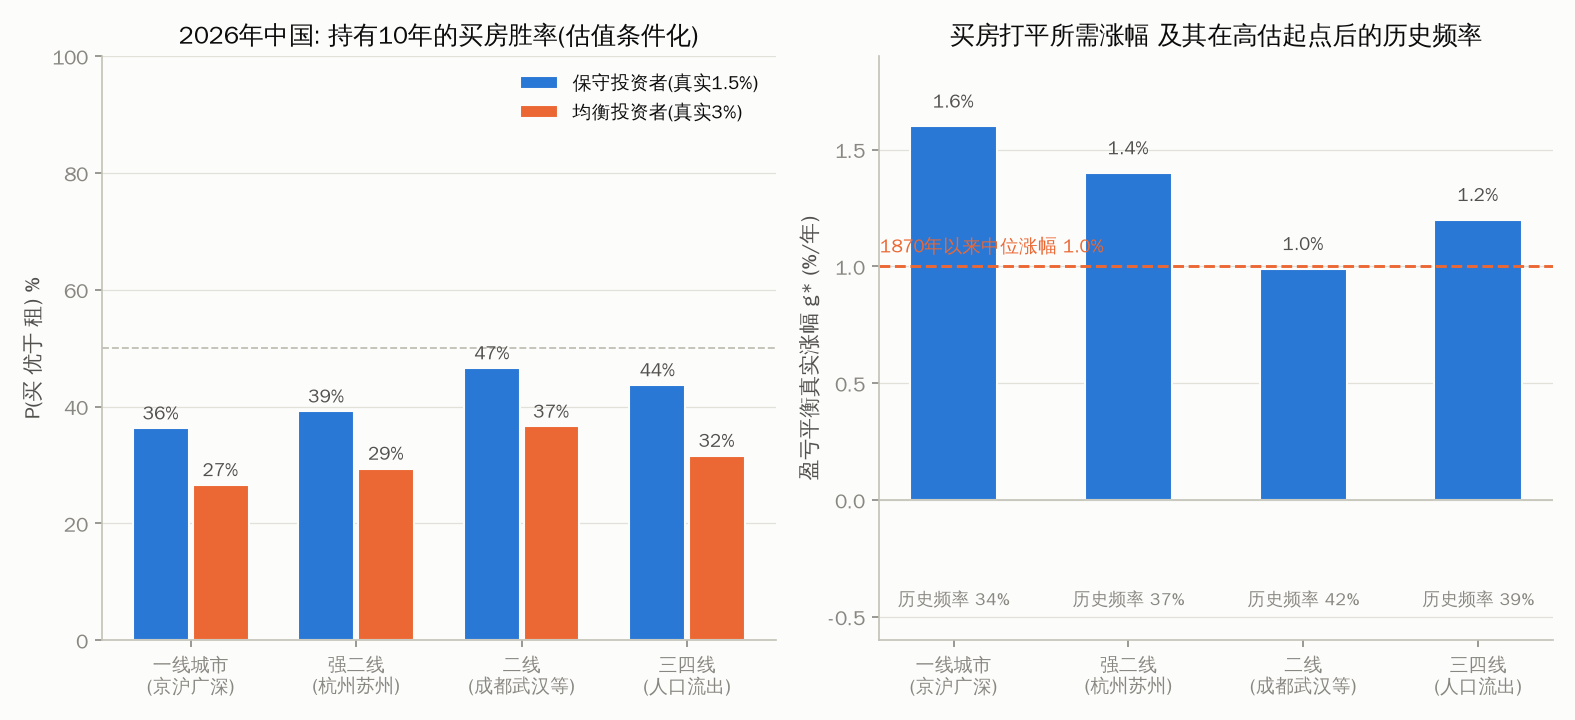
\includegraphics[width=\linewidth]{fig7_china_2026.png}
\caption{2026 年中国四类城市：持有 10 年的买房胜率（左）与盈亏平衡涨幅及其历史频率（右）。}
\end{figure}

\begin{table}[H]\centering\footnotesize
\begin{tabular}{lcccc}
\toprule
持有10年 & 一线(京沪广深) & 强二线(杭苏) & 二线(成都武汉等) & 三四线(人口流出) \\
\midrule
当前租金收益率 & 1.8\% & 2.0\% & 2.4\% & 2.2\% \\
盈亏平衡真实涨幅 g* & +1.6\%/年 & +1.4\%/年 & \textbf{+1.0\%/年} & +1.2\%/年 \\
历史频率(高估组条件化) & 34\% [26, 43] & 37\% [29, 45] & 42\% [35, 50] & 39\% [32, 47]* \\
P(买优于租)·保守投资者 & 36\% [28, 45] & 39\% [32, 48] & \textbf{46\% [39, 54]} & 44\% [37, 51]* \\
P(买优于租)·均衡投资者 & 26\% [18, 35] & 29\% [21, 38] & 37\% [28, 46] & 32\% [23, 40]* \\
财富差中位(保守, 占房价) & $-$10\% & $-$7\% & \textbf{$-$2\%} & $-$5\%* \\
90\% 区间(保守) & [$-$43\%, +60\%] & [$-$41\%, +62\%] & [$-$37\%, +67\%] & [$-$39\%, +65\%]* \\
\bottomrule
\end{tabular}
\end{table}

*三四线数字失真，见下文场外修正。方括号为 95\% 区间（以国家为整群自助）。

\textbf{读表须知：相邻城市档之间的区间大幅重叠。}一线 36\% [28, 45] 与二线 46\% [39, 54] 有交集，强二线与二线几乎完全重叠。本表支持的是\textbf{梯度}（租金收益率越高越偏买）而不是\textbf{排序}；能被数据分开的是两端。

\textbf{所有城市、所有口径都在 50\% 以下——2026 年在中国买房的金融账仍偏租，但已远离 2021 年的一边倒。}历史频率层给出 34\%--42\%，全量求值层给出 26\%--46\%，两条独立的路到达相近的答案。

\textbf{二线省会最接近打平，且是唯一``不赌涨价''的画像。}租金收益率 2.4\% 对上 3.1\% 的按揭，盈亏平衡涨幅恰好落在历史中位数（+1.0\%）上；胜率 46\%（区间 [39, 54]，四档中唯一上沿越过 50\% 的）、财富差中位仅 $-$2\% 房价。压力表同样显示：二线横盘十年亏 10\% 房价；一线横盘亏 17\%，日本路径（$-$2\%/年）亏 36\%。

\textbf{三四线的 44\% 是系统性高估。}模型假设期末能以市价、1.5\% 成本卖出，这在人口流出城市不成立；把卖出成本提到 5\% 后，横盘十年亏 16\%、日本路径亏 34\%。三四线的房子应按\textbf{耐用消费品}估值——``这个价格买来住二十年，转售价值按零计，还合算吗''。

\textbf{日本参照——估值信号会被体制切换压倒。}本文数据中的日本：1990 年起的十年真实房价年化 \textbf{$-$2.2\%}；1995 年起 \textbf{$-$3.6\%}；2000 年按估值已落入``低估组''，其后十年仍是 \textbf{$-$3.2\%}。人口下行叠加通缩的体制里，均值回归信号连续失效二十年。中国 2026 与日本 1992--94 的相似处（人口负增长、通缩压力、高库存）与不同处（核心城市已先跌 20--30\%、城镇化仍有余量、按揭利率已在低位）都摆在明面上。本文不裁决中国走哪条路径，只把两条路径的后果都算出来：\textbf{历史中位路径下，2026 年在中国多数城市买房接近打平；日本路径下，任何城市买房都亏掉三成上下的房价。}你对``中国是不是日本''的判断，就是你的答案里最大的那个变量。

\textbf{估值分组是假设，不是数据。}条件化需要每个城市``过去 25 年的常态租金收益率''，而中国没有公开的城市级长序列。本文取的常态值（一线与强二线 2.4\%、二线 2.8\%、三四线 3.0\%）是判断，因此报告其影响：下表给出每个城市落入中间组的\textbf{门槛}（常态低于该值即不再属于高估组），以及三种分组下的保守投资者胜率。

\begin{table}[H]\centering\footnotesize
\begin{tabular}{lccccc}
\toprule
城市 & 常态假设 & 落入中间组的门槛 & 高估组（正文口径） & 中间组 & 不分组 \\
\midrule
一线城市(京沪广深) & 2.4\% & 2.05\% & 36\% [28, 45] & 46\% [38, 57] & 45\% [39, 50] \\
强二线(杭州苏州) & 2.4\% & 2.28\% & 39\% [32, 48] & 50\% [41, 59] & 47\% [42, 52] \\
二线(成都武汉等) & 2.8\% & 2.74\% & 46\% [39, 54] & 54\% [46, 63] & 53\% [48, 57] \\
三四线(人口流出) & 3.0\% & 2.51\% & 44\% [37, 51] & 51\% [43, 61] & 50\% [45, 55] \\
\bottomrule
\end{tabular}
\end{table}

\textbf{二线的常态假设 2.8\% 距其门槛 2.74\% 只有 6 个基点}——若成都、武汉的常态略低于 2.8\%，该档就落入中间组，胜率从 46\% 升到 54\%。所有敏感性都朝同一方向：放松高估假设只会让买方更有利，正文的高估组口径是\textbf{对买方最保守}的一端。因此``二线可以买''不依赖这个假设（两种分组下胜率都在四六开之间），而``一线偏租''依赖于``一线常态租金收益率高于 2.05\%''——读者若掌握本地长序列，应以之替换本文的假设值重算。

\subsection{分人群建议}

以下建议由上表的金融账推导，非金融因素作为方向性修正。先立四条与城市无关的红线：

\begin{enumerate}\itemsep0.2em
\item \textbf{预期持有期不足 5 年，不买。}交易成本摊薄压倒其他一切变量（4.6 节）。
\item \textbf{月供超过税后收入 40\%，不买。}月供是每个月都要赢的账；被迫中途卖出会把 90\% 区间的左尾（$-$30\% 到 $-$40\% 房价）变成现实。
\item \textbf{掏空应急储备去凑首付，不买。}买房最大的个体风险不是房价，是被迫在坏时点卖出。
\item \textbf{只买现房或二手，不碰高风险期房。}期房折价买的是开发商的信用，不是房子。
\end{enumerate}

\textbf{25--35 岁、居住城市未定：默认租。}持有期不确定直接触发红线 1。特别对一线城市：月供是同等房屋租金的 \textbf{2.0 倍}（房价 100 的房子年租 1.8、年供 3.6），\textbf{是房东在补贴租客}。租房+定投攒首付在金融账上严格占优。

\textbf{30--45 岁、定居城市已定——分城市：}
\begin{itemize}\itemsep0.2em
\item \textbf{二线省会（租金收益率 $\geq$2.3\%）：可以买。}唯一``打平只需历史平均涨幅''的画像（胜率 46\%，区间 [39, 54]；财富差中位 $-$2\%），横盘亏 10\% 在有稳定收入的家庭承受范围内。定居确定+持有 10 年以上+月供合规，金融账不再构成反对理由。
\item \textbf{一线与强二线：金融账仍偏租（胜率 27\%--39\%），但代价已缩小到可被非金融因素合理买断。} 2021 年买房的期望代价是 30\%+ 房价，2026 年缩小到中位约 7\%--9\%——学区、户口、``不被房东赶''的稳定感，现在有了一个可量化的价格。但买前自检：日本路径下亏 36\% 房价，对首付三成的家庭即是\textbf{净值腰斩以上}。
\item \textbf{三四线（人口流出）：按耐用消费品逻辑。}房价便宜到``住二十年、残值归零也比租便宜''的，买；否则租——人口流出城市的租金只会越来越便宜。
\end{itemize}

\textbf{45--60 岁：问题从``买不买''变成``仓位''。}中国城镇家庭资产约六到七成已在房产。\textbf{不加仓}——第二套投资房的账（租金收益率 2.0--2.4\% 对比 1.73\% 国债）补偿不了空置、折旧、流动性与集中度风险；\textbf{置换可以做}；\textbf{考虑减仓}——多套房家庭利用核心城市成交回暖的窗口把流动性最差的那套变现，是本节确定性最高的一条。\textbf{60 岁以上：不新增任何房产杠杆}，余房处置宜早不宜晚——接盘你房子的 25--45 岁人口，未来二十年每年都比今年少。

\textbf{收入维度}：低收入家庭（月供触红线 2）在任何城市都先租，为``上车''买远郊新房是最差选择。高收入家庭的金融账结论不变；唯一提醒是集中度——年收入十倍以上压在单一城市的单一资产上，无论胜率是 45\% 还是 68\%，都不是任何组合理论会推荐的配置。

\textbf{一句话矩阵：}

\begin{table}[H]\centering\small
\begin{tabularx}{\textwidth}{lXXX}
\toprule
 & 一线/强二线 & 二线省会 & 三四线 \\
\midrule
25--35 流动期 & \textbf{租}（房东在补贴你） & 租，除非定居已定 & 租 \\
30--45 定居期 & 金融账偏租（代价约一成房价）；非金融因素强且压力自检过再买 & \textbf{可买}（唯一不赌涨价、金融账打平的画像） & 按消费品逻辑：便宜就买，不便宜就租 \\
45--60 配置期 & 不加仓；置换可做 & 不加仓；置换可做 & \textbf{减仓} \\
60+ & 核心区自住，余房早处置 & 同左 & 同左 \\
\bottomrule
\end{tabularx}
\end{table}

\subsection{二因素速查表：查你自己的格子}

前文的全部机器可以压缩成一张两维的表——\textbf{纵轴是你所在城市的租金收益率（年租金$\div$房价），横轴是预期持有年数}。一个因素值得当轴，必须既影响大、又\textbf{在读者之间差异大}（基准：二线画像，$g^*$ 对各因素的敏感度）：

\begin{table}[H]\centering\footnotesize
\begin{tabularx}{\textwidth}{lXXX}
\toprule
因素 & 对 $g^*$ 的影响 & 2026 年读者之间的差异 & 处理方式 \\
\midrule
租金收益率 & 每 1pp 移动 $g^*$ 约 $-$1.1pp & 跨城市 1.5\%--5\%+ & \textbf{表格纵轴} \\
持有期 & 10$\to$5 年 +0.4pp；10$\to$20 年 $-$0.3pp & 因人 3--20 年不等 & \textbf{表格横轴} \\
按揭利率 & 每 1pp 移动 $g^*$ 约 \textbf{+0.64pp} & LPR 统一定价，人与人只差约 $\pm$0.15pp & 当作常数（3.1\%）；LPR 变动超过 $\pm$0.5pp 时表格作废重算 \\
租方投资收益率 & 每 1pp 移动 $g^*$ 约 +0.47pp & 因人而异且难以自知 & \textbf{稳健带}：每格对真实 1.5\% 与 3\% 两档同时计算，两档同向才给结论 \\
工资/租金涨幅 & 每 1pp 只移动 $g^*$ 约 $-$0.11pp（租金基数仅为房价的 2\% 上下） & 城市间约 $\pm$1pp & 量级小，且已由联合抽样覆盖；工资另经``月供 $\leq$40\%''红线起作用 \\
\bottomrule
\end{tabularx}
\end{table}

下表每格给出（保守投资者胜率/均衡投资者胜率）与判定，其余参数同 8.1 节：

\begin{table}[H]\centering\scriptsize
\setlength{\tabcolsep}{3.5pt}
\begin{tabular}{llccccc}
\toprule
年租金$\div$房价 & 2026 年参照 & 持有3年 & 5年 & 10年 & 15年 & 20年 \\
\midrule
$\leq$1.5\% & 一线核心区、深圳部分板块 & \textbf{租} (36/31) & \textbf{租} (41/36) & \textbf{租} (40/33) & \textbf{租} (44/30) & \textbf{租} (44/28) \\
2.0\% & 京沪均值、杭州苏州 & \textbf{租} (40/35) & 中性 (46/40) & 中性 (47/38) & 中性 (52/39) & 中性 (53/37) \\
2.5\% & 成都武汉档二线 & 中性 (45/40) & 中性 (51/45) & 中性 (54/45) & 中性 (61/48) & 中性 (65/47) \\
3.0\% & 少数高收益率城区/县域 & 中性 (50/45) & 中性 (56/50) & 中性 (63/52) & \textbf{买} (71/57) & \textbf{买} (78/58) \\
4.0\% & 美国多数都会区 & \textbf{买} (60/55) & \textbf{买} (66/61) & \textbf{买} (78/69) & \textbf{买} (85/79) & \textbf{买} (91/83) \\
$\geq$5.0\% & 高租金收益率海外市场 & \textbf{买} (71/66) & \textbf{买} (75/72) & \textbf{买} (88/84) & \textbf{买} (94/90) & \textbf{买} (96/93) \\
\bottomrule
\end{tabular}
\end{table}

格内数字的 95\% 区间约 $\pm$7 个百分点，因此\textbf{判定边界上的格子不必当真}，表格能可靠区分的是两端。\textbf{``中性''不是``随便''，而是``金融账不裁决''}：胜率在四六开之间，此时由非金融因素与压力自检定夺。8.3 节的四条红线优先于本表。表格失效条件：按揭利率相对 3.1\% 变动超过 $\pm$0.5 个百分点、开征持有环节房产税（每 1\% 税率约等价于把你所在的行上移一行）、或你所在城市人口快速流出（下修一档）。

\section{局限}

\begin{enumerate}\itemsep0.2em
\item \textbf{体制依赖（可切换，且已检验）。}历史分布混合了金本位、战争管制、战后信贷扩张与低利率时代。算法支持限定样本期（\texttt{History(since=1950)}），本文默认全样本以保守为先。只用战后窗口时，\textbf{无条件}频率整体右移约 7 个百分点（画像 A：22\%$\to$29\%）；但\textbf{按估值条件化之后，高估组几乎不动}（画像 A 的胜率 20\%$\to$21\%，第 8 节四类中国城市 $-$1.2 到 $-$1.5 个百分点），体制效应只在中、低估值组存在（画像 B 60\%$\to$68\%，画像 C 38\%$\to$48\%）。\textbf{本文最依赖的判断——高估值市场买房不划算——对样本期不敏感；反倒是对买方有利的判断，部分依赖战后体制的延续。}
\item \textbf{窗口重叠（已修正，但不彻底）。}回归显著性以双向聚类标准误报告（t 从 $-$5.05 降到 $-$2.08），全部频率与胜率以国家为整群配 95\% 区间。残余问题：block 只有 16 个；整群法假定国家之间独立，而全球房价周期违反这一假定——真实区间只会比本文报告的更宽。
\item \textbf{年化常数近似。}以窗口年化速率代替路径，低估了含杠杆买方的中途被迫卖出风险与再融资选择权，两者方向相反，净效应未定。
\item \textbf{测度。}历史租金序列平滑、品质调整不完全；跨国房价指数口径差异。
\item \textbf{买的是一套房，不是全国指数。}个人承担的是单套住宅相对指数的特异性波动，完全不在窗口数据里。算法提供开关（\texttt{run(..., idio\_sd=)}），但本文\textbf{不估计}这个波动率。把它开到年化 0\%--15\%：

\begin{table}[H]\centering\small
\begin{tabular}{lcccc}
\toprule
特异性年波动率 & 0\% & 5\% & 10\% & 15\% \\
\midrule
画像 A 胜率 & 20\% & 23\% & 27\% & \textbf{31\%} \\
画像 A 财富差中位 & $-$32\% & $-$32\% & $-$32\% & \textbf{$-$32\%} \\
画像 A 财富差 5\% 分位 & $-$113\% & $-$114\% & $-$118\% & \textbf{$-$124\%} \\
画像 B 胜率 & 60\% & 60\% & 60\% & 59\% \\
画像 B 财富差 5\% 分位 & $-$61\% & $-$62\% & $-$67\% & $-$73\% \\
\bottomrule
\end{tabular}
\end{table}

特异性风险\textbf{并不}系统性利好租房：它把胜率拉向五五开（画像 A 从 20\% 升到 31\%），而\textbf{财富差中位数纹丝不动（$-$32\%）}，左尾明显变厚。这暴露了 P(买优于租) 作为决策统计量的缺陷：\textbf{在期望明确为负的市场里，加大不确定性会让胜率变好看}——赢面上升的方式和买彩票一样。这正是本文始终把财富差的中位数与 90\% 区间和胜率并列输出的原因。
\item \textbf{未定价因素。}居住稳定性、搬迁选择权、强制储蓄、学区等捆绑品、负资产的心理成本——本文只算金融账，这些项应作为对概率输出的个人化修正，而非借口无视金融账。
\item \textbf{中国参数的制度调整。} 70 年使用权的续期规则、房产税的开征时点与税率仍是悬置的 C 层变量——房产税每 1\% 税率约等价于把租金收益率永久下调 1 个百分点，足以翻转 8.2 节的多数结论。
\item \textbf{幸存者偏差。}进入窗口统计的 16 国全部是活到 2020 年的发达经济体，经历过革命、没收、恶性通胀的国家要么不在库中，要么最坏年份被剔除规则移出。本文的历史分布是\textbf{存活者的分布}，左尾比真实的全球经验更薄；本文报告的每一个买房胜率都应读作偏高而非偏低。
\end{enumerate}

\section{结论}

买房还是租房是一道算术题，但其中三个变量属于未来。本文给出一个不假装知道未来的算法：可观察的量精确代入，半可预测的量用估值条件化，不可知的量用 150 年跨国历史的经验分布代言，输出买房胜率与财富差分布。实证确认：住房长期回报的主体是租金而非涨价；真实房价长期涨幅的历史中位数只有约 1\%/年；期初租售比是方向可靠但力度温和的预测变量。

对个体读者，结论压缩成三句话：\textbf{先查你所在城市的租金收益率——它决定了你买房是在收租还是在赌涨价；再算出你需要的涨幅在历史上的出现频率——让 150 年的数据代替你对未来的信心喊话；持有期不足五年就不要买。}其余的，是概率——而且是带着 $\pm$5--8 个百分点区间、只能读到十位数的概率。20\% 与 60\% 之间的差别是数据能支撑的，20\% 与 25\% 之间的差别不是。一个诚实的买租工具，既要拒绝给出点估计的涨幅预测，也要拒绝假装自己的概率精确到个位。

\section*{参考文献}

\begin{itemize}\itemsep0.2em
\item Campbell, S., M. Davis, J. Gallin, and R. Martin (2009). ``What Moves Housing Markets: A Variance Decomposition of the Rent-Price Ratio.'' \emph{Journal of Urban Economics} 66(2).
\item Gallin, J. (2008). ``The Long-Run Relationship between House Prices and Rents.'' \emph{Real Estate Economics} 36(4).
\item Himmelberg, C., C. Mayer, and T. Sinai (2005). ``Assessing High House Prices: Bubbles, Fundamentals and Misperceptions.'' \emph{Journal of Economic Perspectives} 19(4).
\item Jordà, Ò., K. Knoll, D. Kuvshinov, M. Schularick, and A. M. Taylor (2019). ``The Rate of Return on Everything, 1870--2015.'' \emph{Quarterly Journal of Economics} 134(3).
\item Jordà, Ò., M. Schularick, and A. M. Taylor (2017). ``Macrofinancial History and the New Business Cycle Facts.'' \emph{NBER Macroeconomics Annual} 31.
\item Knoll, K., M. Schularick, and T. Steger (2017). ``No Price Like Home: Global House Prices, 1870--2012.'' \emph{American Economic Review} 107(2).
\item Mankiw, N. G., and D. Weil (1989). ``The Baby Boom, the Baby Bust, and the Housing Market.'' \emph{Regional Science and Urban Economics} 19(2).
\item Poterba, J. (1984). ``Tax Subsidies to Owner-Occupied Housing: An Asset-Market Approach.'' \emph{Quarterly Journal of Economics} 99(4).
\item Saiz, A. (2010). ``The Geographic Determinants of Housing Supply.'' \emph{Quarterly Journal of Economics} 125(3).
\item Sinai, T., and N. Souleles (2005). ``Owner-Occupied Housing as a Hedge Against Rent Risk.'' \emph{Quarterly Journal of Economics} 120(2).
\end{itemize}

\subsection*{第 8 节 2026 年中国数据来源（2026 年 8 月检索）}

\begin{itemize}\itemsep0.2em
\item LPR 与房贷利率：新华社/中国政府网：2026-08-20 LPR 维持不变（1 年期 3.0\%、5 年期以上 3.5\%）\url{https://english.www.gov.cn/archive/statistics/202608/20/content_WS6a8692ecc6d00ca5f9a0cb78.html}；人民日报海外版：房贷利率又迎下调（存量公积金利率 2026-01-01 起下调，5 年以上首套 2.6\%）\url{https://paper.people.com.cn/rmrbhwb/pc/content/202601/08/content_30130383.html}；CEIC：个人住房贷款加权平均利率（2026 年 3 月 3.06\%）\url{https://www.ceicdata.com/en/china/rediscount-and-lending-rate/cn-lending-rate-weighted-average-individual-housing-loan}
\item 租金收益率与租售比：证券时报：一线城市住宅平均租金由跌转涨，50 城住宅平均租售比回升（京沪广深 1.64\%/1.95\%/1.87\%/1.82\%，二线 2.36\%）\url{https://www.stcn.com/article/detail/3920236.html}
\item 房价走势：中指研究院：2026 上半年中国房地产市场总结与下半年趋势展望（百城二手累跌 2.9\%、核心城市企稳）\url{https://www.cih-index.com/news/2026-07-09/54872544.html}
\item 利率环境：CEIC：中国 10 年期国债收益率（2026-07 约 1.73\%）\url{https://www.ceicdata.com/zh-hans/china/pbc--ccdc-treasury-bond-and-other-bond-yield-daily/bond-yield-treasury-bond-10-year}；北大国发院：促进物价合理回升——货币政策的困境（低通胀下真实利率偏高）\url{https://www.nsd.pku.edu.cn/docs/2025-12/50c5191a9ca842f88079c50135535aa4.pdf}
\end{itemize}

\end{document}
